%&LaTeX
% !TEX encoding = UTF-8 Unicode
\documentclass{article}
\usepackage{listings}
\lstset{ language = Java}
\usepackage[utf8]{inputenc}
\usepackage[francais]{babel}
\usepackage[T1]{fontenc}
\usepackage{textcomp}
\usepackage[colorlinks=true, linkcolor=black, urlcolor = blue]{hyperref}

\usepackage{graphicx}
\usepackage{ulem}
\usepackage{color}
\usepackage[top=2cm,bottom=2cm,left=2.5cm,right=2.5cm]{geometry}


\definecolor{color01}{rgb}{0.00,0.00,0.00}
\definecolor{color02}{rgb}{0.40,0.40,0.40}
\definecolor{color03}{rgb}{0.07,0.33,0.80}



\title{\Huge{AGETAC\\
Aide à la GEstion TACtique\\}
\huge{{\color{color02} \textit{Document de développement}}}}

\date{Mai 2012}
\author{Projet Agetac - Université de Rennes 1\\
Encadré par Noël Plouzeau}



\begin{document}


\maketitle
\tableofcontents
\newpage


\section{Introduction}

\subsection{Présentation du document}

Le présent document s'adresse aux futurs développeurs ou chargés 
de maintenance de Agetac. Il présente de manière détaillée la procédure à 
suivre pour pouvoir récupérer les fichiers sources du projet, explique brièvement 
l'architecture des fichiers et enfin il montre comment modifier ou ajouter des 
fonctionnalités.

\subsection{GitHub}

Dans tout projet conséquent, la gestion des documents, des versions 
et des mises à jour posent souvent problème. Dès la mise en place 
du projet Agetac, nous avons choisi d'utiliser GitHub, un service qui permet d'héberger 
des projets libres pour gérer les sources et les documents relatifs au projet.

Tous les documents, sources, et exécutables sont téléchargeables 
à cette adresse : \\ \url{https://github.com/Agetac}

\section{Installer l'environnement}


\subsection{Java}

Le projet a été exclusivement développé dans le langage Java. 
Le choix de ce langage a été fait depuis le départ pour des raisons de portabilité. Java 
est également un langage libre, dont la communauté est très active sur Internet.


\subsection{Android}

Le projet à été développé pour fonctionner sur tablette tactile 
Android utilisant la version 3.0.


\subsection{Les librairies utilisées}

\subsubsection{Jackson}

Nous avons intégré à Restlet l'extension Jackson pour la communication 
entre le serveur et les tablettes. Jackson est une librairie très rapide qui permet 
de sérialiser des objets Java en JSON de façon standard, et inversement de convertir 
du JSON en objets Java.

\subsubsection{DataNucleus}

Il s'agit d'un projet open-source qui offre des librairies permettant 
l'accès aux données utilisant des API standards pour un grand nombre de banque 
de données. Nous utilisons donc DataNucleus pour gérer notre modèle de persistance 
qui est JDO (Java Data Object) avec notre système de gestion de données.

\subsubsection{HSQLDB}

Cette librairie nous permet de manipuler notre système de gestion 
de base de données  relationnelles (RDBMS - Relational DataBase Management System 
) Java du même nom.

\subsubsection{ModelMapper}

ModelMapper est un framework de mapping d'objet intelligent qui 
élimine le besoin de mapper les objets manuellement les uns aux autres dans la 
persistance.

\subsubsection{HttpClient et HttpCore de Apache}

Ces librairies nous offrent un support plus robuste du protocole 
HTTP que les packages Java basiques. With Restlet's default HTTP client we had 
problems getting the Client/Server communication work. It seems that either Android 
or the Restlet's default HTTP client cannot handle correctly the chunked transfer 
encoding, which is enabled by default in Restlet's default HTTP client (and there 
is no obvious way to disable it!).

\section{Structure du projet / Rôle des classes}

\subsection{Model}


\subsubsection{Diagramme de classe}

\begin{figure}[htbp]
\begin{center}
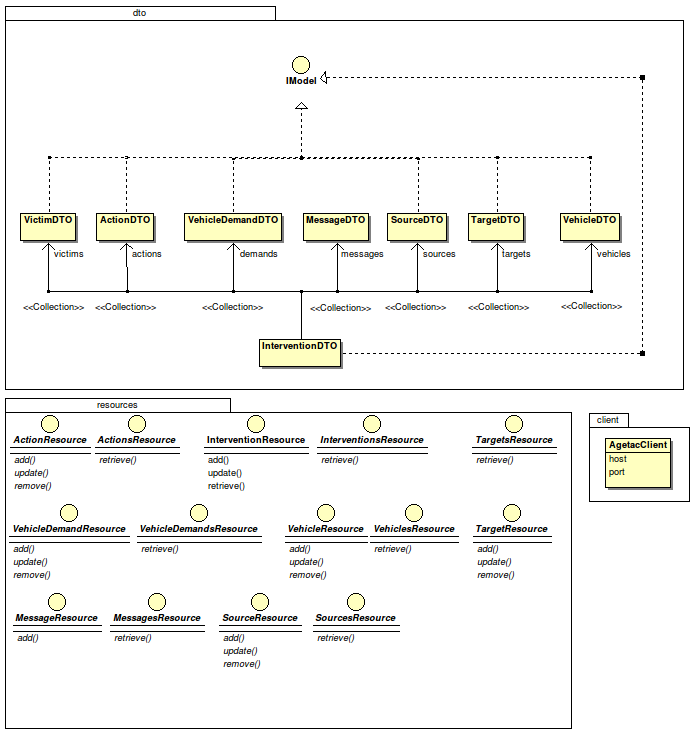
\includegraphics[width=494pt, height=521pt]{doc_dev-fig001.png}
\caption{This should be the caption for \texttt{doc\_dev-fig001.png}.}
\end{center}
\end{figure}

\subsubsection{Description}

\paragraph{Package resources :}

Contient toutes les interfaces des ressources ainsi que les classes 
du package ``resources''que le serveur doit implémenter.

\paragraph{Package observer :}

Contient la classe MyObservable qui étend java.util.Observable 
et qui rend publique la méthode setChanged().

L'intérêt du pattern Observer est de prévenir les classes observatrices 
via un « signal » d'un changement sur les classes observées afin d'effectuer 
une action relative à ce changement.

Ce pattern est utilisé principalement dans le client pour mettre 
à jour les données.

\paragraph{Package dto :}

Ces classes représentent des ressources, « typeDTO.java », 
qui sont amenées à être échangées entre la tablette cliente et le serveur. 
Ce sont ces objets qui transitent sur le réseau. We don't send the ORM entities 
down the wire because, unless we're very careful, there is a risk to pull in a 
lot more of the reachable object tree than what we would like, when Jackson serializes 
an ORM entity (in order to make it pass through the network).

\paragraph{Package client :}

« AgetacClient.java » est une classe ``protocolaire''connaissant 
les opérations GET, POST, PUT à effectuer sur les différentes ressources (telle 
une demande de véhicule ou l'ajout d'une victime). Les fonctions associées effectuent 
les opérations REST correspondantes : elles créent une ressource typeDTO, à 
laquelle est associée une URI, qui sera envoyée au serveur. The idea was to have 
completely transparent JSON (de)serialisation by using the Automatic 
Conversion extension of the restlet framework. For example, 
using this method, the client can do the following to retrieve a vehicle demand :

\begin{lstlisting}
ClientResource clientResource = new ClientResource("some_url");
try {
  VehicleDemandsResource vehicleDemandsResource = 
     clientResource.wrap(VehicleDemandsResource.class);
  return  vehicleDemandsResource.retrieve();
} finally {
  clientResource.release();
}
\end{lstlisting}

However, using this method to (de)serialize collections of objects 
just doesn't work (so well). Let's take for instance the following scenario: Collection\texttt{<}InterventionDTO\texttt{>} 
on server -\texttt{>} JSON/Restlet -\texttt{>} Collection\texttt{<}LinkedHashMap\texttt{>} 
on the client. That is, server side we want to serialize a collection of InterventionDTOs 
to send to the client. Passing through Restlets Automatic Conversion technique, 
the client finally gets a Collection\texttt{<}InterventionDTO\texttt{>}.

Restlet's JacksonRepresentation uses mapper.readValue(representation, 
targetType.class) to do the work, but type parameters are erased (!), so the return 
type becomes Collection.class, and the call becomes mapper.readValue(representation, 
Collection.class). Jackson does the it can in that case; the serialized InterventionDTO 
looks like a map.

To avoid problems with type erasure, for example for calls that 
return typed Collections of objects, we don't use the Automatic Conversion feature 
of Restlet. Instead, we use Jackson directly and a technique to pass full generics 
type information. For example, a call to the method to get the list of interventions 
is implemented the following way :

%\begin{lstlisting}
%try {
%  Representation repr = clientResource.get();
%  TypeReference<Collection<InterventionDTO>> tr = 
%      new TypeReference<Collection<InterventionDTO>>();
%  ObjectMapper mapper = new ObjectMapper();
%  Collection<InterventionDTO> col = null;
%  col = mapper.readValue(repr.getStream(), tr);
%  return col;
%} catch (Exception e) {
%    e.printStackTrace();
%} finally {
%      clientResource.release();
%}
%\end{lstlisting}

\subsection{Client}

\subsubsection{Diagramme de classe}

\begin{figure}[htbp]
\begin{center}
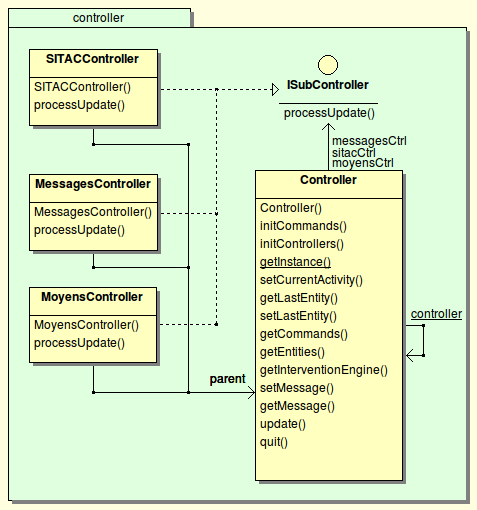
\includegraphics[width=357pt, height=382pt]{doc_dev-fig002.png}
\caption{This should be the caption for \texttt{doc\_dev-fig002.png}.}
\end{center}
\end{figure}


\parindent=0pt
Le \textbf{Controller} est en relation avec les différentes \textbf{XXXActivity} et le moteur de l'application.

C'est un singleton qui observe les changements des différentes Activity et qui appel en conséquence le contrôleur associé à l'activité.

Le contrôleur observe aussi le moteur \textbf{InterventionEngine.} Lorsque celui-ci se met à jour, le contrôleur se charge d'appeler la méthode \textbf{update()} propre à l'activité de type \textbf{ITabActivity} courante.

Chaque sous-contrôleur \textbf{ISubController} correspond à une \textbf{ITabActivity} et sait comment traiter les informations en fonction de l'état de la variable de type \textbf{ActionFlag.}

\begin{figure}[htbp]
\begin{center}
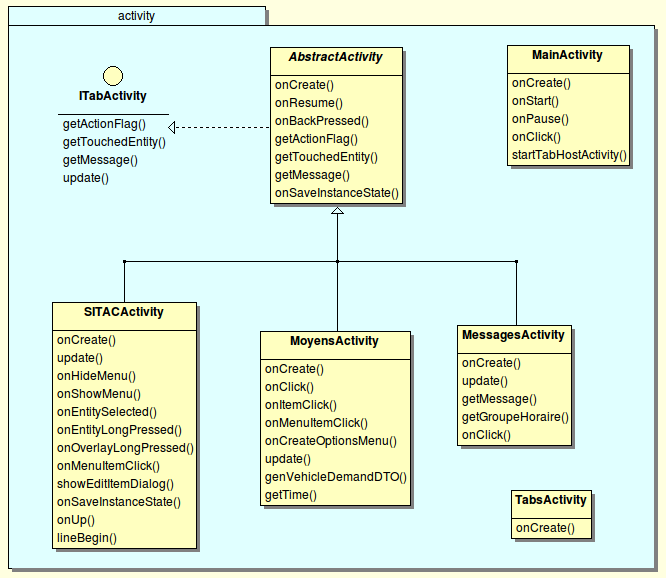
\includegraphics[width=499pt, height=433pt]{doc_dev-fig003.png}
\caption{This should be the caption for \texttt{doc\_dev-fig003.png}.}
\end{center}
\end{figure}


Les Activity forment l'interface graphique de l'application. Elles 
jouent aussi le rôle de ``listener''en réagissant aux interactions de l'utilisateur. 
Aussi elles définissent un \textbf{ActionFlag}
approprié pour l'action en cours (ajout, suppression, update, ..., ainsi qu'une 
\textbf{IEntity} courante (touchedEntity). Enfin, elles notifient à leur observateur quand leur état a changé.

\begin{figure}[htbp]
\begin{center}
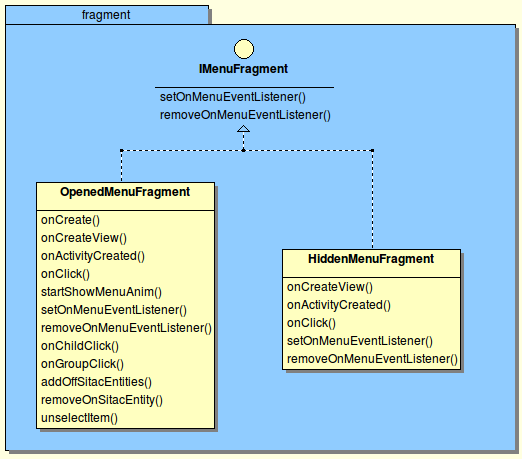
\includegraphics[width=391pt, height=344pt]{doc_dev-fig004.png}
\caption{This should be the caption for \texttt{doc\_dev-fig004.png}.}
\end{center}
\end{figure}

Les \textbf{IMenuFragment} sont des menus affichés dans l'onglet SITAC. On a deux menus : 

\begin{itemize}
\item OpenedMenuFragment : menu ouvert sur la SITAC.

\item HiddenMenuFragment : menu fermé sur la SITAC.

\end{itemize}

\parindent=0pt
{ Les menus sont capables de notifier les interactions de l'utilisateur 
via l'interface }{ \textbf{IOnMenuEventListener}}{ . 
Si une classe hérite de cette interface, et s'enregistre comme ``listener''d'un 
}{ \textbf{IMenuFragment}}{ , alors elle recevra 
des events en fonction des actions faites sur le menu.}

\begin{figure}[htbp]
\begin{center}
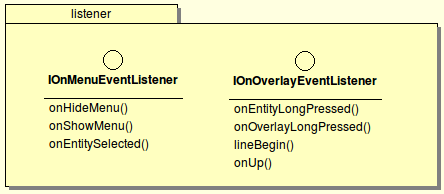
\includegraphics[width=332pt, height=145pt]{doc_dev-fig005.png}
\caption{This should be the caption for \texttt{doc\_dev-fig005.png}.}
\end{center}
\end{figure}

\begin{figure}[htbp]
\begin{center}
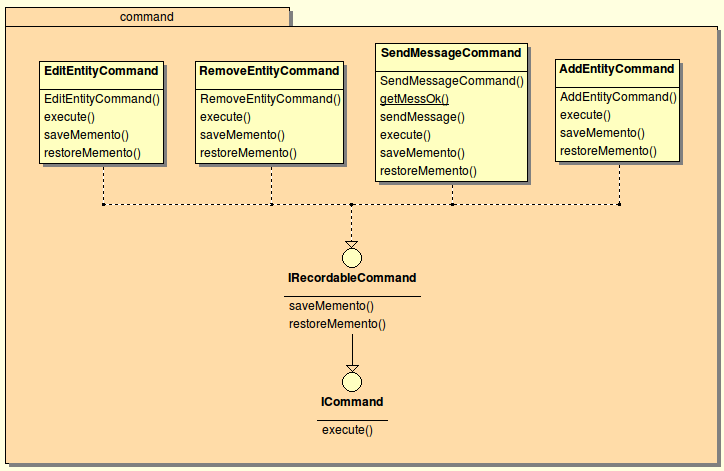
\includegraphics[width=542pt, height=353pt]{doc_dev-fig006.png}
\caption{This should be the caption for \texttt{doc\_dev-fig006.png}.}
\end{center}
\end{figure}

Pattern Command classique permettant de réifier les actions ``client/serveur''possibles 
au sein de l'application.

\begin{figure}[htbp]
\begin{center}
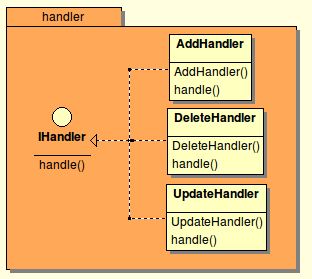
\includegraphics[width=233pt, height=209pt]{doc_dev-fig007.png}
\caption{This should be the caption for \texttt{doc\_dev-fig007.png}.}
\end{center}
\end{figure}

\vspace{13pt}
{ Les }{ \textbf{Handler}}{  prennent 
des }{ \textbf{IEntity}}{  (côté client donc) et 
se chargent d'effectuer les modifications nécessaires pour mettre à jour la liste 
d'entités côté client et côté serveur.}

Ils vont par exemple se charger de supprimer un véhicule côté 
client et donc d'envoyer le message de suppression au serveur via la classe \textbf{AgetacClient}
du model.

Le fait de passer dans un handler va automatiquement déclencher 
une mise à jour côté client de l'interface graphique. Car l'état du moteur 
va changer en fonction de l'action à prendre en charge.

\begin{figure}[htbp]
\begin{center}
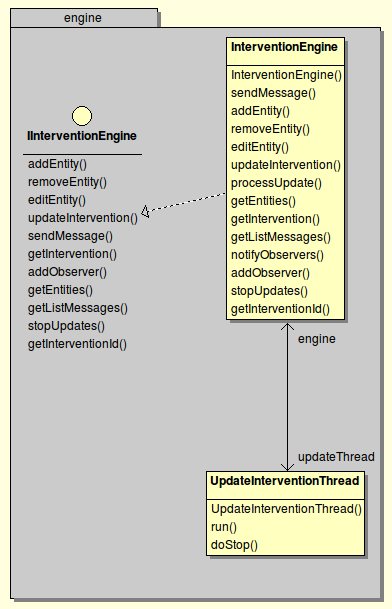
\includegraphics[width=293pt, height=456pt]{doc_dev-fig008.png}
\caption{This should be the caption for \texttt{doc\_dev-fig008.png}.}
\end{center}
\end{figure}

Le moteur de l'application se charge de la connexion entre le 
client et le serveur. Il transmet les messages aux \textbf{Handler}
en ce qui concerne les actions possibles (REST).

L' \textbf{UpdateInterventionThread} quant à lui, va se charger d'appeler la méthode \textbf{updateIntervention()}
périodiquement ? afin de mettre à jour le client avec les informations récupérées 
sur le serveur.

Lorsque l'état du moteur change (donc quand sa liste d'entités est modifiée), il va notifier le contrôleur.

\begin{figure}[htbp]
\begin{center}
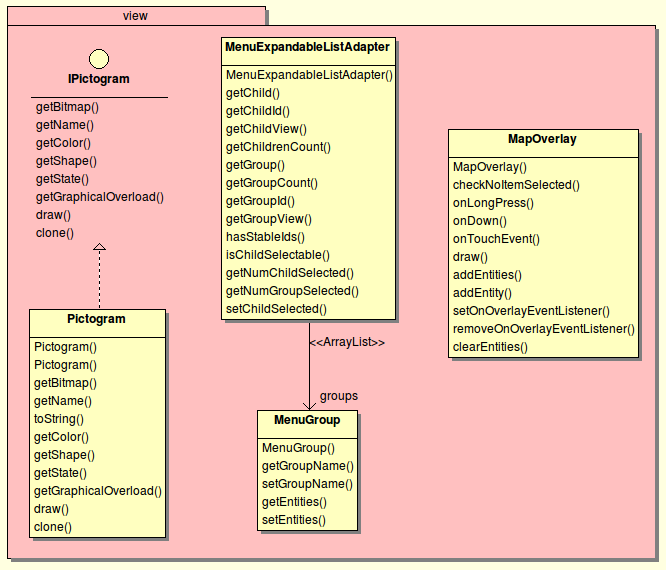
\includegraphics[width=499pt, height=427pt]{doc_dev-fig009.png}
\caption{This should be the caption for \texttt{doc\_dev-fig009.png}.}
\end{center}
\end{figure}


\textbf{MapOverlay} représente la carte de 
la SITAC. Il est capable de dessiner les différentes entités sur la carte et 
déclenche des évènements lorsque l'utilisateur interagi avec.

Le \textbf{MenuExpandableListAdapter} permet de dessiner les différentes entités dans le menu.

Un \textbf{Pictogram} est une image et est associé à une \textbf{Entity}
et un \textbf{IModel.}

\begin{figure}[htbp]
\begin{center}
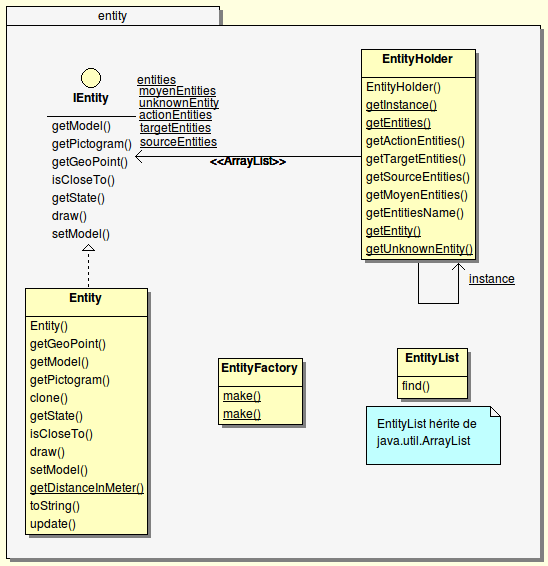
\includegraphics[width=410pt, height=424pt]{doc_dev-fig010.png}
\caption{This should be the caption for \texttt{doc\_dev-fig010.png}.}
\end{center}
\end{figure}

Les \textbf{IEntity} sont des objets qui contiennent un \textbf{IModel } et un \textbf{IPictogram.} Ils peuvent être dans différent états durant leur cycle de vie :

\begin{itemize}

\item[EntityState.MENU : ] une entité du menu, vide, qui sert de base ``clonable''.

\item[EntityState.ON\_SITAC : ] une entité avec un modèle bien défini et une position connue.

\item[EntityState.OFF\_SITAC : ] une entité avec un modèle bien défini mais une position inconnue (elle apparaîtra donc dans l'onglet ``Position à définir'' du menu).

\end{itemize}

\subsubsection{Description}

\subsection{Serveur}

\subsubsection{Diagramme de classe}

\begin{figure}[htbp]
\begin{center}
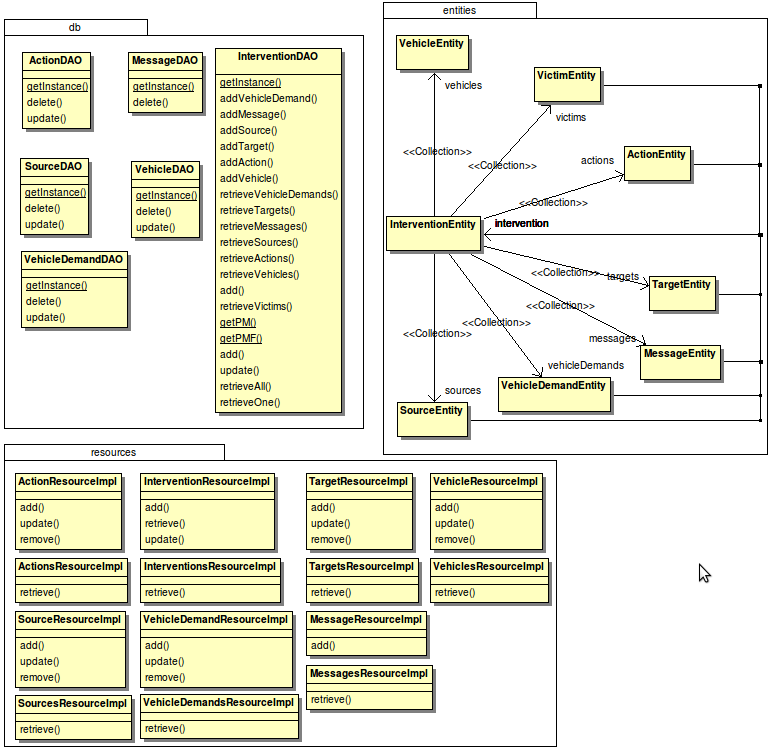
\includegraphics[width=526pt, height=509pt]{doc_dev-fig011.png}
\caption{This should be the caption for \texttt{doc\_dev-fig011.png}.}
\end{center}
\end{figure}

\subsubsection{Description}

\vspace{13pt}
\leftskip=0pt
{ L'architecture du serveur est décomposée en une classe principale 
et quatre packages.}

\vspace{13pt}
{ La classe « Server.java », qui se situe dans le package principal 
du serveur (org.agetac.server) a pour but d'initialiser le serveur et de lui associer 
un }{ \textit{Router}}{ .}

{ L'initialisation du serveur consiste en la création d'un }{ \textit{Restlet 
component }}{ sur le protocole HTTP et le port 8888 auquel nous 
associons une }{ \textit{application. }}{ L'interêt 
des }{ \textit{Restlet components}}{  résident dans 
le fait de pouvoir héberger plusieurs }{ \textit{applications}}{  
ayant des fonctionnalités très différentes, tel qu'un client HTTP et un client 
SMTP par exemple, au sein d'une même JVM (Java Virtual Machine). Le but est de 
fournir une alternative portable, flexible et totalement orientée REST à l'API 
Servlet standard.}

{ Une fois l'application créée, il faut lui associer un }{ \textit{Router}}{ . 
Un }{ \textit{Router }}{ est un objet Restlet permettant 
d'associer des URI (Uniform Resource Identifier) à des ressources Restlet avec 
lesquelles la tablette cliente communiquera. Nous utilisons plusieurs templates 
d'URI :}

\leftskip=36pt
\parindent=-18pt
{ « /ressources » permet d'obtenir la liste de tous les objets 
du type ressource sur le serveur.}

{ « /ressource/\{ressourceId\} »  permet d'obtenir un objet particulier 
du type ressource identifié par l'id ressourceId.}

\leftskip=0pt
\parindent=0pt
{ Ces deux templates d'URI sont combinés au sein du serveur sur 
chaque ressource pour obtenir par exemple la liste des objets de type ressource2 
au sein d'un objet particulier de type ressource1 : « /ressource1/\{ressource1Id\}/ressources2 
».}

{ Toutes les URI sont associées à des classes d'implémentation 
de ressources situés dans le package ``resources''}

\vspace{13pt}
{ \textbf{Le package ``entity''}}

{ Chaque classe dans ce package est de la forme « typeEntity.java 
» et représente un type de base avec toutes les fonctions get() et set() associées 
: InterventionEntity, MessageEntity, etc ...Ces classes sont annotées pour pouvoir 
être persistantes et ont pour unique but d'être stockées.}

\vspace{13pt}
{ \textbf{Le package ``db''}}

\vspace{13pt}
{ In this package we have classes that implement the DAO (Data Access 
Object) pattern. A typical DAO provides an interface that defines its contract 
with the outside world. This takes the form of a series of data access and data 
update methods. }

\vspace{13pt}
{ We defined our DAOs as interfaces. This has various benefits, 
and the one we highlight here is that we can now provide an implementation using 
DataNucleus and JDO (in the following paragraph we give a quick review of JDO). 
We could, in principle, provide a DAO implementation of this interface using JDBC 
for example, or one for whatever persistence technology. It demonstrates a flexible 
design strategy allowing components to be swapped at a future date.}

\vspace{13pt}
{ As mentioned in the previous paragraph, in the Agetac server, 
we use Java Data Objects (JDO) for persistence, a standard interface for storing 
objects containing data into a database. The standard defines interfaces for annotating 
Java objects, retrieving objects with queries, and interacting with a database 
using transactions. }

\vspace{13pt}
{ An application that uses the JDO interface can work with different 
kinds of databases without using any database-specific code, including relational 
databases, hierarchical databases, and object databases. The Agetac server uses 
a simple HSSQL database but, as with other interface standards, JDO simplifies 
porting the application between different storage solutions.}

\vspace{13pt}
{ The standard procedure for implementing DAO methods using JDO, 
is to retrieve a PersistenceManager , obtain a transaction, and perform our operations 
(create, retrieve, update, delete). Due to space constraints, we do not outline 
in detail those steps.}

\vspace{13pt}
{ - enhancing data classes}

\vspace{13pt}
{ JDO uses a post-compilation \texttt{"}enhancement\texttt{"} step 
in the build process to associate data classes with the JDO implementation. There 
a Datanucleus Plugin for Eclipse does this step automatically when building, but 
not everyone can use this approach because it requires administrative rights to 
install it or a local Eclipse installation. In our approach, we created an ant 
script that performs the enhancement (DataNucleus provides an Ant task to enhance 
files).}

\vspace{13pt}
{ - fetch groups}

\vspace{13pt}
{ Another thing to note is the use of fetch groups. When the Android 
client requests an Intervention, he wants not only the primitive fields of an intervention 
(id, name), he also wants the related vehicles, messages, targets, etc. Consequently, 
when we bring an intervention from the database, we also have to bring the related 
entities. We define the related entities to fetch with the use of fetch-groups. 
In our project, fetch groups are defined using Java annotations.}

\vspace{13pt}
{ - problematic updates}

\vspace{13pt}
{ One way to update an object with JDO is to fetch the object, then 
modify it while the PersistenceManager that returned the object }{ \textit{is 
still open}}{ . Changes are persisted when the PersistenceManager 
is closed. However, in the case of a client/server application, that doesn't work. 
}

\vspace{13pt}
{ In a client/server application typically we retrieve an object, 
we send it to the client for some processing, and then the client it back and the 
server is supposed to persist the changes. By the time the object is returned to 
the server for persisting the changes, the persistent manager that initially retrieved 
the object }{ \textit{is gone}}{ .}

\vspace{13pt}
{ To mitigate this problem, when the server is called to update 
an object, we search for that object in the database and, if found, we map (using 
the ModelMapper library) the fields of the sent object to the fields of the retrieved 
object.}

\vspace{13pt}
{ \textbf{Le package resources}}

{ Ce package contient deux classes par type de ressource : une classe 
permettant de travailler sur une instance particulière de la ressource, « typeResourceImpl.java 
», et une classe permettant de travailler sur la liste de toutes les instances 
de cette ressources, « typesResourceImpl.java ».}

Chaque classe étend ServerResource de l'API Restlet et implémente 
son interface contenue dans le Model, « typeResource » ou « typesResources ». 
Ces classes implémentent les fonctions add(), remove() et update() permettant 
d'ajouter, de supprimer ou de mettre à jour la ressource. Ces fonctions prennent 
en entrée un objet typeDTO (Data Transfer Object) envoyé par les tablettes clientes 
et mettent à jour la persistance.

\vspace{13pt}
{ \textbf{Le package client}}

Il s'agit d'une IHM (Interface Homme Machine) permettant d'interagir 
directement avec les informations contenues sur le serveur. Ce package est articulé 
autour de trois sous-packages, « controller », « model » et « view » permettant 
de décomposer cette IHM selon le pattern MVC.

Le pattern MVC (Modèle Vue Contrôleur) est un pattern qui organise 
la conception d'une IHM : le modèle gère ou décrit les données, la vue correspond 
à l'interface direct avec laquelle l'utilisateur interagit et le contrôleur prend 
en charge la synchronisation et la mise à jour du modèle et de la vue.


\section{Fonctionnement}


\begin{figure}[htbp]
\begin{center}
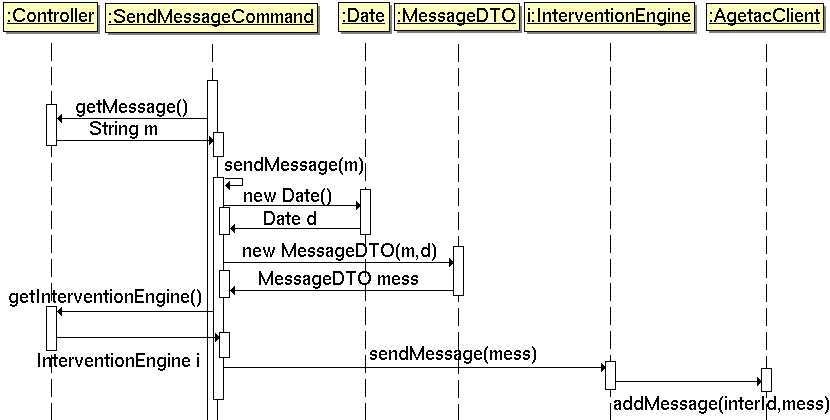
\includegraphics[width=531pt, height=268pt]{doc_dev-fig012.png}
\caption{Envoi message côté client.}
\end{center}
\end{figure}

\begin{figure}[htbp]
\begin{center}
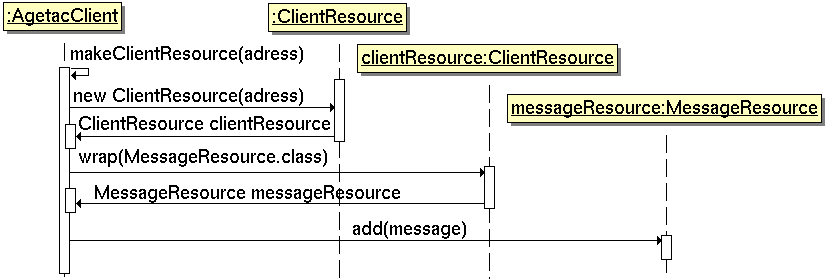
\includegraphics[width=515pt, height=172pt]{doc_dev-fig013.png}
\caption{Envoi message côté serveur.}
\end{center}
\end{figure}

\end{document}
